\documentclass[12pt,a4paper,oneside,titlepage]{article}
\usepackage[round, comma]{natbib}               %Zitieren
\usepackage{graphicx}             %Graphik-Paket
\usepackage{subcaption}            %zwei Figures nebeneinander
\usepackage{color}
\usepackage[USenglish]{babel}     %Spracheinstellung USEnglish
\usepackage[utf8]{inputenc}       %Umlaute & Akzente
\usepackage{lmodern}              %Computer-Modern als Vektorgrafiken

\usepackage{setspace}             %Zeilenabstand 1,5
\onehalfspacing
%Zeilenabstand vor und nach Gleichungen ändern
\makeatletter
\g@addto@macro\normalsize{%
  \setlength\abovedisplayskip{2pt}
  \setlength\belowdisplayskip{5pt}
  \setlength\abovedisplayshortskip{0pt}
  \setlength\belowdisplayshortskip{0pt}
}
\makeatother

\usepackage{geometry}             %Seitenränder anpassen
\geometry{a4paper,left=30mm,right=25mm, top=2cm, bottom=3cm}



\usepackage{microtype}            %besseres Schriftbild
\usepackage{footmisc}             %Fußnoten

\usepackage[tbtags]{mathtools}            %Mathematische Symbole
\usepackage{amsmath, amsthm, amssymb, amsfonts}    %bessere mathematische Formeln

\usepackage{booktabs}             %bessere Tabellen
\usepackage{marvosym}             %Symbole einfügen


\usepackage{titletoc}			  %Inhaltsverzeichnis anpassen
\dottedcontents{section}[3em]{\bfseries}{2.9em}{1pc}
\dottedcontents{subsection}[4em]{}{3.3em}{1pc}

\usepackage[small]{titlesec}     %Überschriften anpassen

\usepackage{epstopdf}            %include Matlab Figures


\renewcommand{\thesection}{\Roman{section}}  %Römische Zahlen bei Überschrift
\renewcommand{\thesubsection}{\thesection.\Roman{subsection}}





\begin{document}
\parindent 0pt %kein Erstzeileneinzug
\begin{titlepage}
	\centering
	
\includegraphics[width=0.8\textwidth]{pictures/LogoFU}\par\vspace{1cm}
	{\scshape\large Freie Universität Berlin \par}
	\vspace{1cm}
	{\scshape\large Seminar Paper in "Recent Research in Macroeconomics"\par}
	\vspace{1.5cm}
	{\LARGE\bfseries Replication of Erceg \& Lindé (2012):\par}
	\vspace{0.5cm}
	{\Large\bfseries Is there a Fiscal Free Lunch in a Liquidity Trap?\par}
	\vspace{2cm}
	{\Large\itshape Denis Maciel \& Tobias Müller\par}
	\vfill
	supervised by\par
	Prof. Dr. Mathias \textsc{Trabandt}

	\vfill

% Bottom of the page
	{\large \today\par}
\end{titlepage}


\doublespacing
\tableofcontents

\pagebreak[4]
\listoffigures
\listoftables
\newpage

\section{Introduction}

The financial crisis in 2007/08 and the following worldwide recession marked a turning point in the economic and public debate about optimal fiscal and monetary policy. In the aftermath of the great recession, economists discussed about the effectiveness of expansionary fiscal policy to stabilize the economy and stimulate the private sector. In this debate the fiscal multiplier has received special attention.

In the the aftermath of the crisis, governments and central banks launched unconventional and in part uncharted measures to mitigate the harmful consequences of a prolonged recession. The strong reduction in the nominal interest rate was very preeminent among those measures because many central banks reduced the interest rates down to zero. Since the zero lower bound was hit and monetary policy exhausted one of its main tools, fiscal policy became more relevant. This new state of affair gave birth to a literature increasingly concerned with fiscal policy and the government spending multiplier. This literature stresses the effectiveness of government spending in cases where monetary policy has already brought interest rates to zero.
\par
\bigskip
In this context, the authors Christopher Erceg and Jesper Lindé address in the paper \textit{"Is there a Fiscal Free Lunch in a liquidity trap?"} the question whether policymakers should limit the size of the government spending. They do so by writing a model in which the liquidity trap is endogenously determined and then calculating the multiplier schedule for different calibrations. They also draw the very important distinction between marginal and average spending multiplier, which is crucial for policymakers to better understand the effects of changes in government spending. Finally, the paper provides new insights into how fiscal spending and austerity impact the government budget in a liquidity trap.
\par
\bigskip
In our paper, we try to replicate the basic results of \citet{Erceg.2014} using Dynare. It is organized as follows. In Section II, we discuss briefly the current literature about the government spending multiplier and explain the main results of the analyzed paper. In Section III, we concentrate on the key equations of the paper, explain the structure of the model and the underlying microeconomics of the simple New Keynesian model. In Section IV, we present the results of the impulse response to show how the model reacts to an exogenous consumption taste shock and government spending hike. We also give some impressions on how the results vary if we change the slope of the Phillips curve or the parameters of the monetary rule. In Section V, we dive deeper into the concept of multiplier and explain the distinction between \textit{marginal} and \textit{average} multiplier. We show that the variation of the fiscal multiplier depends highly on the size of the government response and on the average contract duration (the Calvo parameter). In Section VI, we analyze the impacts of the increase in government spending on the government budget and answer the question wether there is a fiscal free lunch in a liquidity trap. In Section VII we provide some additional information on our workflow that could be useful for future participants of this seminar. In Section VIII, we conclude with final remarks.


\section{Fiscal Policy and the Spending Multiplier }

Before the financial crisis in 2007/08, fiscal policy was often seen as inefficient and costly. In particular, the time-lag of the implementation of the fiscal spending and the crowding-out effect on the private sector were seen as great obstacles to the use of public spending programs. Besides the theoretical economic arguments, different models have delivered contrasting results on the effects of fiscal policy. \citet{CoenenG..2010} and \citet{Afonso.2010} compare various state-of-the-art macroeconomic models and show the wide range of different frameworks in which the spending multiplier can be analyzed. The type, design, duration and funding of the fiscal stimulus are as important as the circumstances of the economic meltdown, the interaction with monetary policy and the scope for public finance. \citet{Coenen.2010} mention that an economic crisis normally has negative consequences for the current debt position of a country, as we could observe during the euro crisis, and thus the budgetary room for maneuver can be highly at risk in a situation when fiscal packages can normally be extraordinary effective.
\par
\bigskip
New evidence on recent model-based economic research provide some new understanding whether fiscal policy can be an adequate response in a deep recession. \citet{Eggertsson.2011} suggests that stimulating short run aggregate demand, rather than the supply side of the economy, has particularly positive effects at the zero lower bound. \citet{Davig.2009} and \citet{Christiano.2011} show that an increase in government spending can outsize the effect on output in a deep recession, especially in prolonged liquidity traps. Once the nominal interest rate hits the lower bound, there can be a strong case for a fiscal stimulus on a temporary basis to jump-start the economy and push it out of an economic downward spiral.
\par
\bigskip
The key question of the paper "Is there a fiscal free lunch in a liquidity trap?" concentrates on the magnitude of the government spending multiplier, the distinction between marginal and average effects and the impact of the fiscal policy on the government budget.
The paper uses a simple New Keynesian model to analyze the impulse response of two different exogenous shocks. It shows that fiscal policy can play a crucial role in stabilizing the economy during an economic crisis. One important result of the paper is that the marginal multiplier is high in a liquidity trap, but decreases quickly when the size of the government spending increases. We replicate the concept of the marginal spending multiplier, which is a step function depending on the level of government spending.
We also show that under certain conditions, an expansionary fiscal policy can in fact reduce government debt and thus be self-financing, which can be considered a fiscal free lunch. Finally, we point out the risks of fiscal austerity measures while the economy faces a liquidity trap.


\section{The Model}
In this section we describe and summarize the baseline illustration of the New Keynesian dynamic stochastic general equilibrium (DSGE) model \citet{Erceg.2014} use in their paper.\footnote {Additional information and a more detailed derivation of the standard log-linearized version of the New Keynesian model can be found in the Online Appendix of the original paper.} The New Keynesian DSGE model has a RBC-core, but allows for two inefficiencies, so that shocks can cause deviations from the "natural level": monopolistic competition among firms and the Calvo model of firms' price setting. Therefore, the New Keynesian model addresses the deficits of the RBC-models and makes the more realistic assumptions that prices do not adjust continuously and markets are not perfectly competitive. Consequently, monetary policy can affect the real interest rate, thus has real effects. The microfoundation permits a normative policy analysis.
\subsection*{Households}

The representative household decides the intertemporal consumption demand by maximizing
\begin{equation}
E_t \sum_{j=0}^\infty \beta^j \left\{ \frac{1}{1- \frac{1}{\sigma}} \left(C_{t+j} - C\nu_{t+j}\right)^{1-\frac{1}{\sigma}} - \frac{N_{t+j}^{1+\chi}}{1+\chi} + \mu_0F \left(\frac{MB_{t+j+1}(h)}{P_{t+j}}\right)\right\} \nonumber
\end{equation}
under the constraint\newline
$P_t(1+\tau_{C,t})C_t + B_{G,t} + MB_{t+1} = (1-\tau_{N,t})W_tN_t + (1+i_{t-1})B_{G,t-1} + MB_t - T_t + \Gamma_t, \vspace{0.2cm}$
where 0 $< \beta < 1$ is the discount factor and $E_t$ the rational expectations operator. The utility function depends on the households current consumption $C_t$ as deviation from a “reference level” $C\nu_{t+j}$, where the negative taste shock $\nu_t$ reduces this steady-state level. The taste shock, which is responsibly for triggering the liquidity trap, enters the model in the households utility function and affects the consumption decision of the household. The shock changes the marginal utility of consumption and so the willingness of the households to consume the produced goods.\newline
The utility function also depends inversely on hours worked $N_t$. By assuming that $\mu_0$ is arbitrarily small, changes in real money balances have negligible implications for seignorage in the model. The household's budget constraint implies that the expenditure on goods and net purchases of government bonds $B_{G,t}$ equals the after-tax labor income $ \left(1 - \tau_{N,t} \right) W_tN_t$, minus a lump-sum tax $T_t$, plus a proportional share of the profits $\Gamma_t$ of all intermediate firms. The household's optimal plan needs to satisfy the first order conditions, so that we get
\begin{align}
\vspace{-0.5cm} \left(C_t - C\nu_t\right)^{-\frac{1}{\sigma}}  - \lambda_tP_t \left(1 + \tau_{C,t} \right) = 0,\nonumber\\
-N_t^{\chi} + \lambda_t \left(1 - \tau_{N,t} \right) W_t = 0,\nonumber\\
-\lambda_t + \beta \left(1 + i_t \right) E_t\lambda_{t+1} = 0,\nonumber
\end{align}
and finally the Euler equation
\begin{equation}
\frac {\left(C_t - C\nu_t\right)^{-\frac{1}{\sigma}}}{\left(1 + \tau_{C,t} \right)} = \beta E_t \frac{\left(1 + i_t \right)}{1 + \pi_{t+1}} \frac{\left(C_{t+1} - C\nu_{t+1}\right)^{-\frac{1}{\sigma}}}{\left(1+ \tau_{C,t+1}\right)},
\end{equation}
and the aggregate labor supply relation
\begin{equation}
mrs_t \equiv \frac{N_t^\chi}{\left(C_t - C\nu_t\right)^{-\frac{1}{\sigma}}} = \frac{\left(1 - \tau_{N,t}\right)}{\left(1 + \tau_{C,t}\right)} \frac{W_t}{P_t}.
\end{equation}
The last equation shows that the marginal rate of substitution between consumption and labor must equal the after tax real wage.
We have to mention that in our simple New Keynesian Model we set the sales tax $\tau_{C,t}$ equal to zero to get the same results as in the paper.

\subsection*{Firms}
The production function of the firms is
\begin{equation}
Y_t = K^\alpha N_t^{1-\alpha},\vspace{-0.3cm} \nonumber
\end{equation}
where aggregate capital is fixed, but shares of the aggregate capital stock can be allocated across the firms. All firms choose the factor demand such that costs are minimized. The real factor costs per marginal product therefore are
\begin{equation}
\frac{MC_t}{P_t} = \frac{W_t/P_t}{\left(1 - \alpha \right) K^\alpha N_t^{-\alpha}}.
\end{equation}
The firm, which can reset its price in period t, chooses a price $\left(P_t^{opt} \right)$ and maximizes the problem
\begin{equation}
\max_{P_t^{opt}\left(f\right)} E_t \sum_{j=0}^\infty \xi_p^j \psi_{t,t+j} \left[ \left(1 + \pi \right)^j P_t^{opt}\left(f\right) - MC_{t+j} \right] Y_{t+j} \left(f\right),\nonumber
\end{equation}
where $\psi_{t,t+j}$ is the discount factor and $\xi$ the probability that the firm's price set in t will still be valid in period t+1. The demand function for the good $\left(f\right)$ which faces the firm is given by
\begin{equation}
Y_{t+j}\left(f\right) = \left[\frac{P_t \left(f\right)}{P_t} \right]^{\frac{-\left(1+\theta_p\right)}{\theta_p}} Y_t \nonumber,
\end{equation}
which varies with the relative price of the good, the substitution elasticity $\theta$ and the aggregate demand $Y_t$. The first order condition with optimal price $\left(P_t^{opt} \right)$ is
\begin{equation}
E_t \sum_{j=0}^\infty \xi_p^j \psi_{t,t+j} \left[ \frac{\left(1 + \pi \right)^j P_t^{opt}\left(f\right)}{1 + \theta_p} - MC_{t+j} \right] Y_{t+j}\left(f\right) = 0.
\end{equation}
For deriving the New Keynesian Phillips curve, we also need the average price of the final goods
\begin{equation}
P_t = \left[\left(1 - \xi_p\right)\left(P_t^{opt}\right)^{\frac{-1}{\theta_p}} + \xi_p \left(\left(1 + \pi\right)P_{t-1}\right)^{\frac{-1}{\theta_p}} \right]^{-\theta_p}.
\end{equation}
Finally, we have to derive the aggregate resource constraint
\begin{equation}
C_t + G_t \leq \left(\frac{P_t^*}{P_t}\right)^{\frac{\left(1+\theta_p\right)}{\theta_p}} K^\alpha N_t^{1-\alpha},
\end{equation}
where actual output $Y_t$ can be divided into private consumption and government spending $\left(Y_t \equiv C_t + G_t \right)$.\newline
By log-linearizing the equations (1) to (7) around the steady-state and after some rearranging, we receive the key equations of the model used in the \citet{Erceg.2014} paper.

\subsection*{The Government}

The government budget constraint is given by
\begin{equation}
B_{G,t} = \left(1 + i_{t-1}\right)B_{G,t-1} + P_tG_t - \tau_{C,t}P_tC_t - \tau_{N,t}W_tN_t - T_t - MB_{t+1} + MB_t,  \nonumber
\end{equation}
where after scaling with $1/ P_tY_t$, the left side of the equation defines the end-of-period real government debt. In the model the government can issue bonds to finance the budget. As mentioned before, we set the consumption tax $\tau_{C,t}$ in our simplified model equal to zero for all t. The government charges the labor income with a constant tax rate $\tau_N$ according to the equation \[\tau_N = \frac{g_y}{s_N}\] with $g_y$ as the government share of steady-state output $\left(g_y = 0.2 \right)$ and $s_N$ as the steady-state labor share $\left(s_N = 0.7\right)$.
The government also collects a lump-sum tax $\left(\tau_t \equiv T_t/P_tY)\right)$, which varies in time and is adjusted according to the evolution of the debt stock $\left(\tau_t = \varphi_b b_{G,t-1}\right)$. Therefore, the fiscal policy specifies that taxes respond to government debt, but does not affect other macro variables in the model. We set the tax rule parameter $\varphi_b$ equal to 0.01. Consequently, the evolution of the tax base depends mostly on the variation in labor tax revenues the first years after a negative taste shock. The government budget is zero in steady-state in the simple benchmark model.\newline
Monetary policy follows a Taylor rule which is subject to the zero lower bound
\begin{equation}
i_t = max \left(-i, \gamma_{\pi} \pi_t + \gamma_x x_t\right)  \nonumber.
\end{equation}
By setting the parameters $\gamma_{\pi}$ and $\gamma_x$ arbitrarily large, we assume that the monetary policy would completely stabilizes inflation and the output gap in absence of the the zero lower bound. In the next section, we also consider the alternative case where the parameters of the monetary policy rules are lower.\newline
Table \ref{tab:Tabel1} provides an overview over the parameter values, we use in our benchmark calculation.
\bigskip


\section{Impulse Response}

First, we focus on the impulse response of a large negative taste shock and a positive government spending shock to counteract the fall in output. The main steps to replicate the results of \citet{Erceg.2014} are the following:
\begin{enumerate}
\item Write up the model equations in Dynare and set the parameter values provided in the paper\vspace{-0.3cm}
\item Solve the model without baseline shock, so that the nominal interest rate does not hit the zero lower bound and compute then impulse to government spending and consumption taste shock\vspace{-0.3cm}
\item Impose the ZLB on monetary policy and simulate effects of a large negative consumption demand shock, so that the economy hits the zero lower bound\vspace{-0.3cm}
\item Find the right parameter and shock values for an eight quarter liquidity trap in an environment of an positive government spending shock equal to one percentage point of steady-state output\vspace{-0.3cm}
\item Calculate the difference between the impulse responses of both shocks and the taste shock only to get the effects of the government spending shock
\end{enumerate}
The large taste shock leads to a fall of the potential real interest rate $r^{pot}$. The length of the liquidity trap is defined by how long $r^{pot}$ remains below $-i$.
Figure \ref{IRnoinflation} gives the first impression of how the negative taste shock affects the key variables of the model: the real interest rate, the output gap, inflation and government debt to GDP.
\begin{figure}[th]
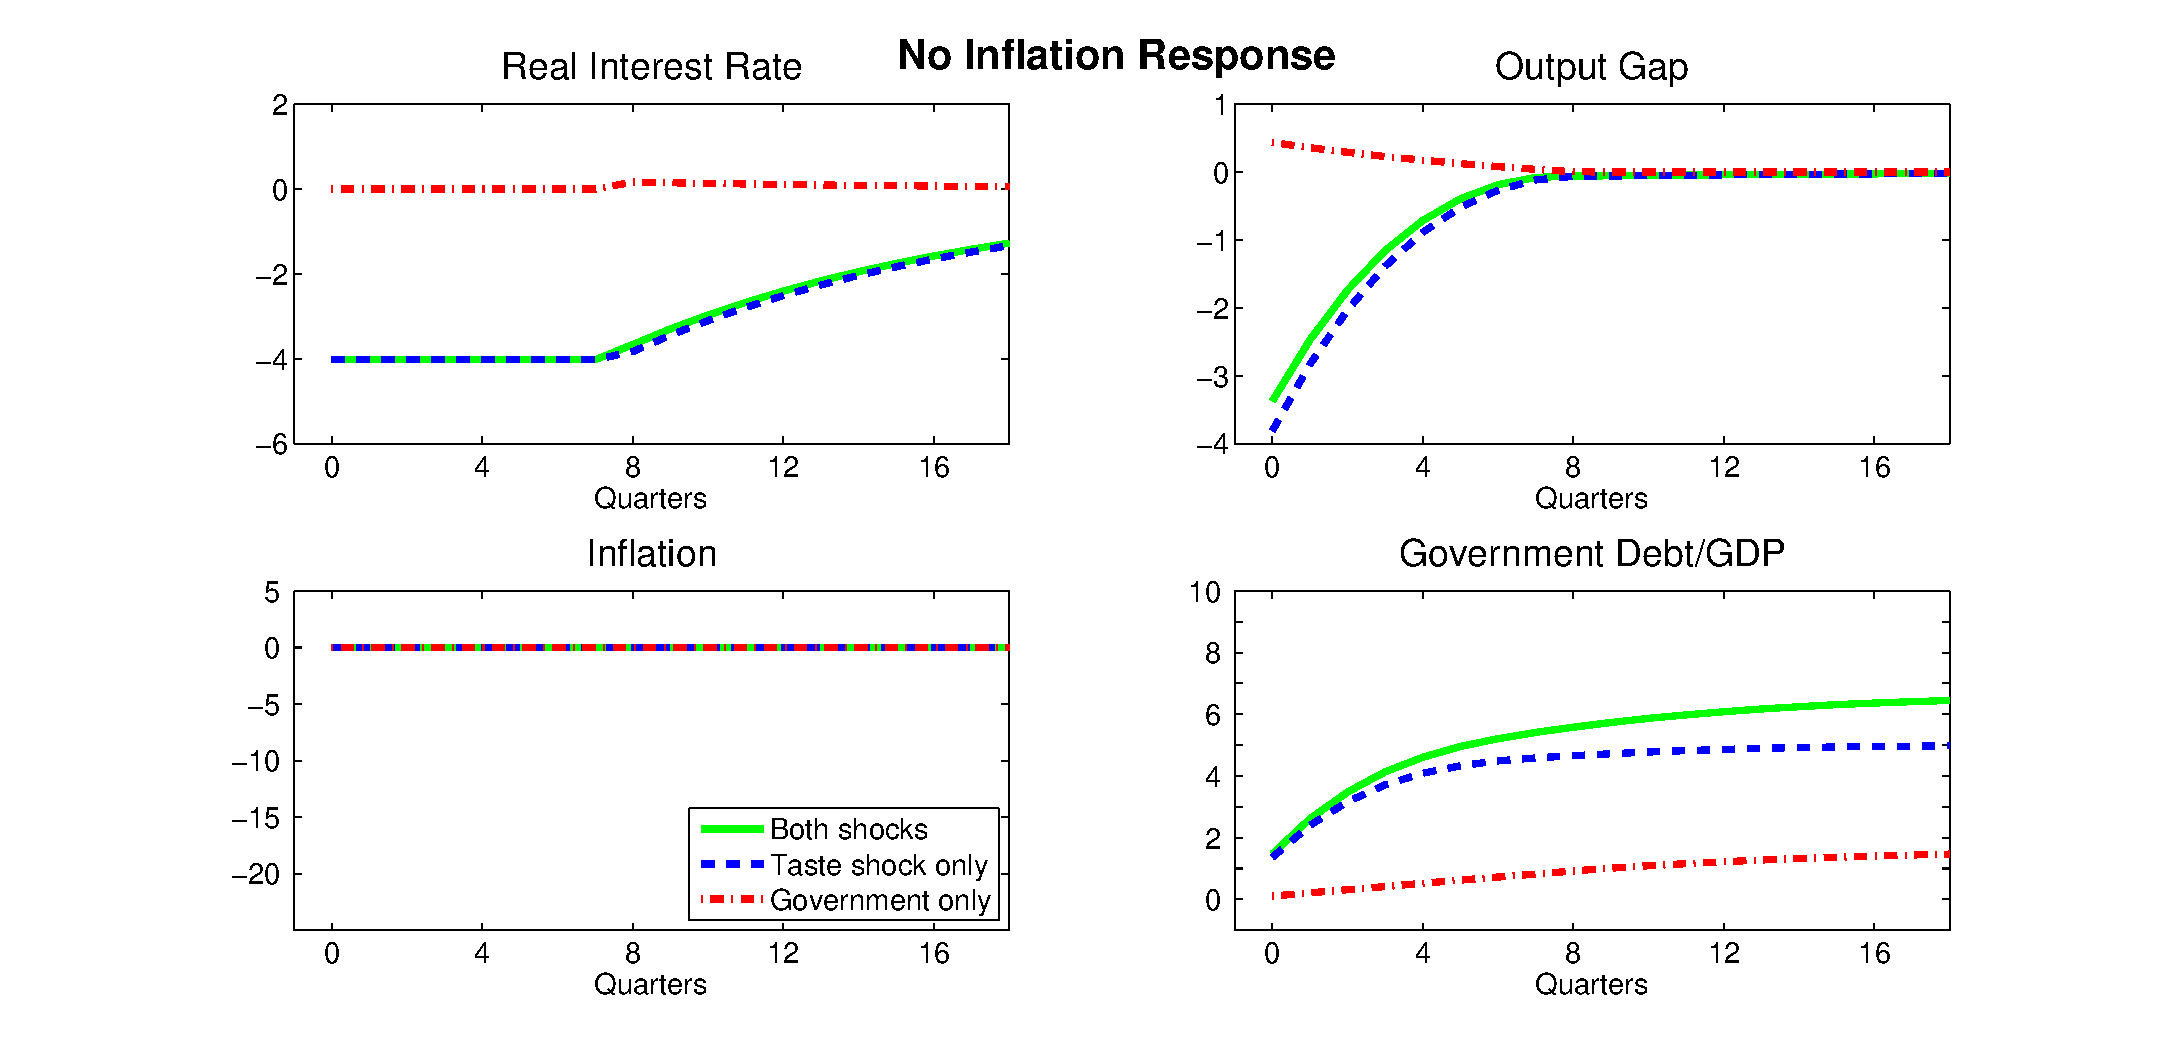
\includegraphics[width=\textwidth]{Paperpics/Figure2noIR}
\caption{Immediate Rise in Government Spending (No Inflation Response)}
\label{IRnoinflation}
\end{figure}

In the following subsections we explain the cruxes to get the right results. We explain more in detail the shock parameters, emphasize the role of the price rigidity and the policy responses to the negative taste shock.


\subsection*{The Shock Parameter}
The model consists of two different types of exogenous shocks: the consumption taste shock and the government spending shock. The adverse consumption shock triggers the fall of the potential real interest rate. We begin the analysis by setting the Calvo parameter equal to one and thus eliminating changes in inflation. For the following calculations and figures, it is important to find the exact values for an eight quarter liquidity trap. The nominal and real interest rate fall simultaneously to the zero lower bound when the adverse consumption shock is large enough. Both interest rates stay at the zero lower bound for eight quarters and return  gradually to the steady state. The negative shock also leads to a fall in output and to a rise in government debt. In Figure \ref{IRnoinflation} to \ref{fig:debt} we simulate the model with a negative taste shock of $29.2$. The taste shock is scaled in the model by the scale parameter $\nu_c$ and $\left(1- g_y\right)$, which can be seen as the private sector’s share of the steady-state output. Therefore, the negative taste shock can be interpreted as $0.01 * \left(1-0.2\right) * 29.2 = 0.2336$ or a $23,36\%$ fall in output of steady-state GDP.
\par
\bigskip
To counteract the negative effects on output, the government increases spending by one percentage point of total GDP. The interpretation of the government spending shock is similar to the taste shock.  The government shock is scaled by the government share of total output $g_v$. We simulate the model with a spending increase of $0.05$. This leads after scaling $0.2 * 0.05 = 0.01$ to the required government spending shock.
In Figure \ref{IRnoinflation} the solid green line shows the dynamic effects of both shocks, the blue dashed line the result of the negative taste shock without the rise in spending and the red dash-dotted line the isolated effects of the government shock in the scenario of both shocks. It is important to mention that the red line is calculated by subtracting the results of the simulation of the taste shocks only from the results of the simulation of both shocks to isolate the effects of the government spending rise.
\par
\bigskip
Figure \ref{Figure1b} shows the consequences for the potential real interest rate when we loop the negative taste shock between $0$ and $50$ and then calculate the duration of the liquidity trap.
The step function implies that a sightly larger adverse shock does not change the liquidity trap duration. Only when the potential real interest rate falls beyond a certain threshold, the adverse taste shock extends the liquidity trap duration.

\begin{figure}[!th]
\centering
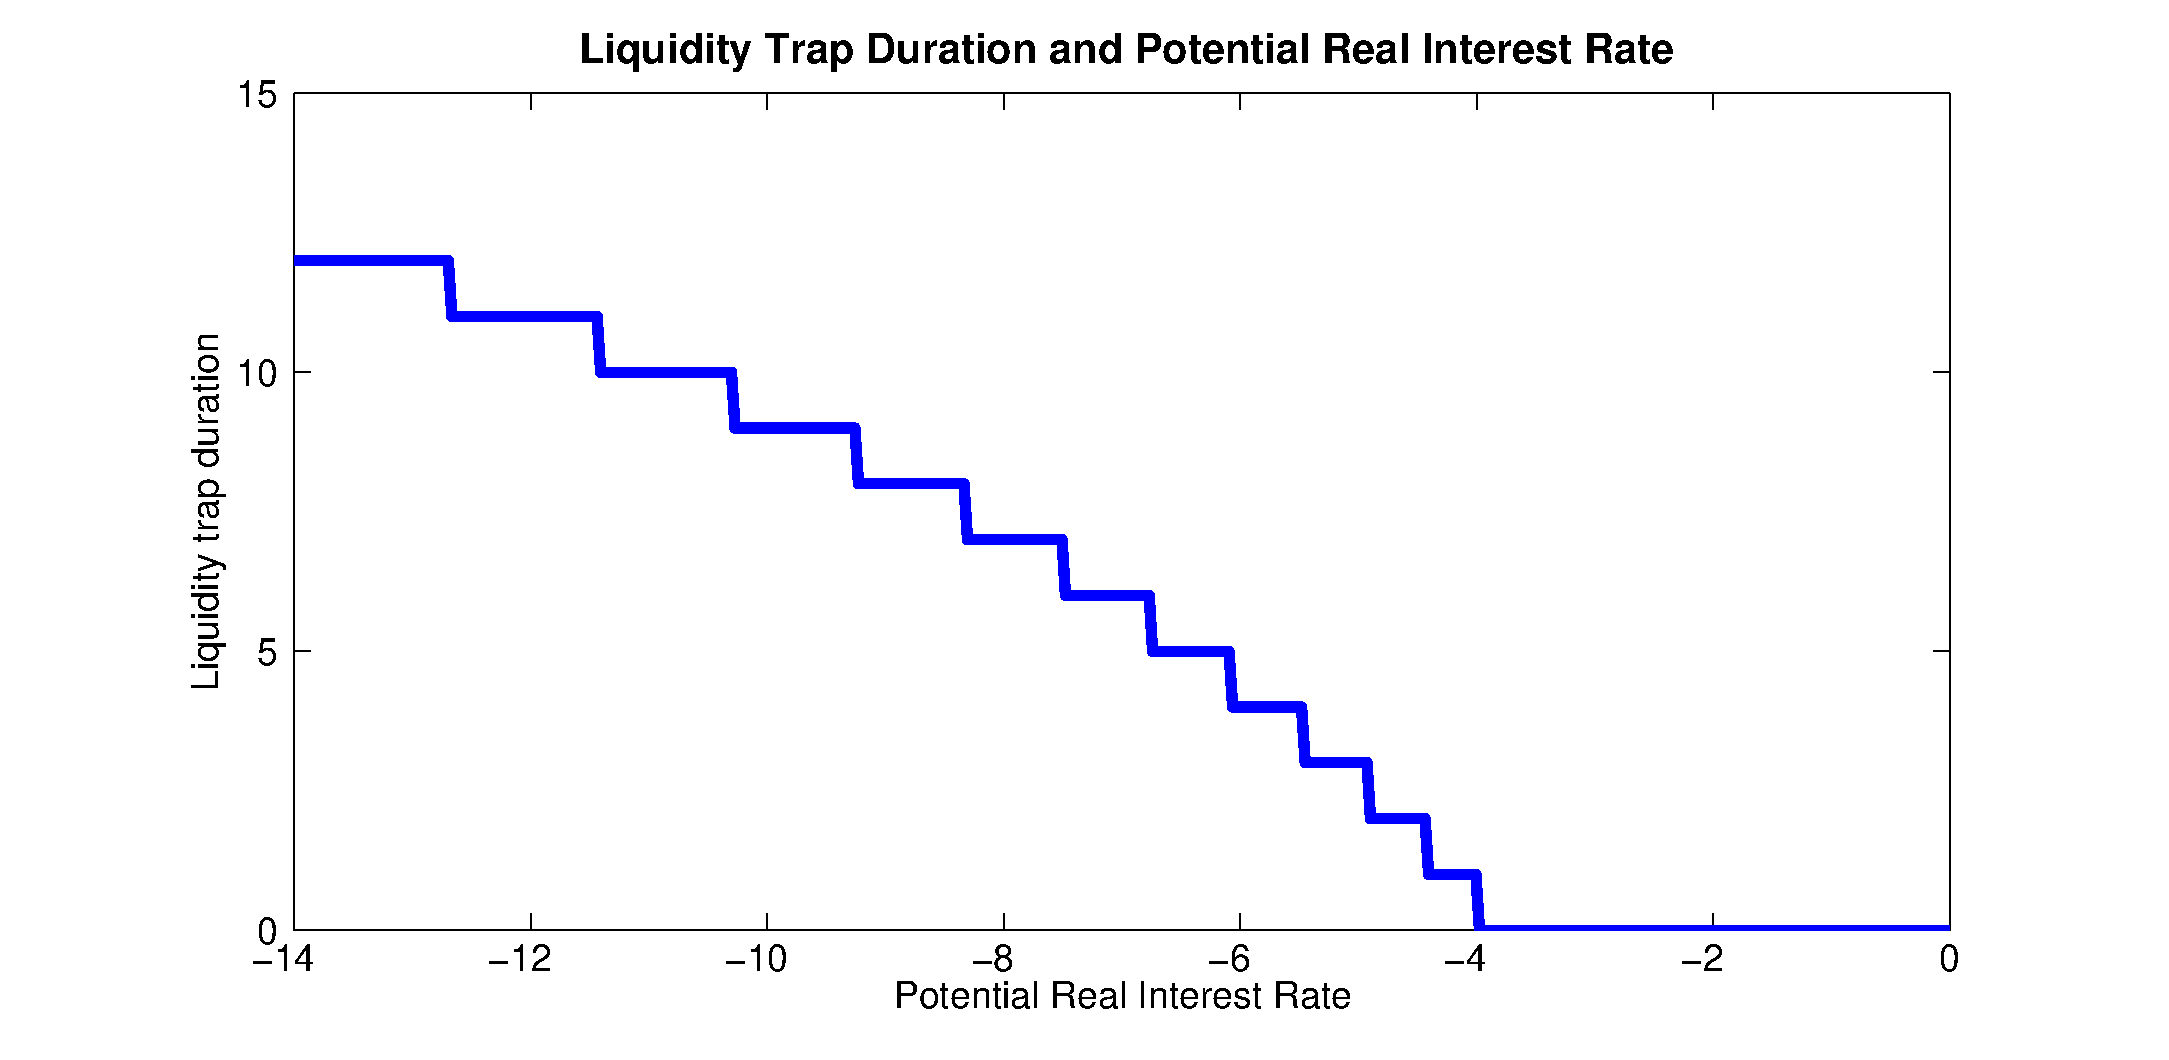
\includegraphics[width=0.8\textwidth]{Paperpics/Figure1b}
\caption{Potential Real Interest Rate and Variation of Taste Shock}
\label{Figure1b}
\end{figure}

Figure \ref{Figure1bscatter} shows the scatter plot of the adverse taste shock. We loop the taste shock between the starting point $0$ and the end point $50$ with the increment of the sequence of $0.1$ and show the 501 shocks which enter the model to create the step function.

\begin{figure}[!th]
\centering
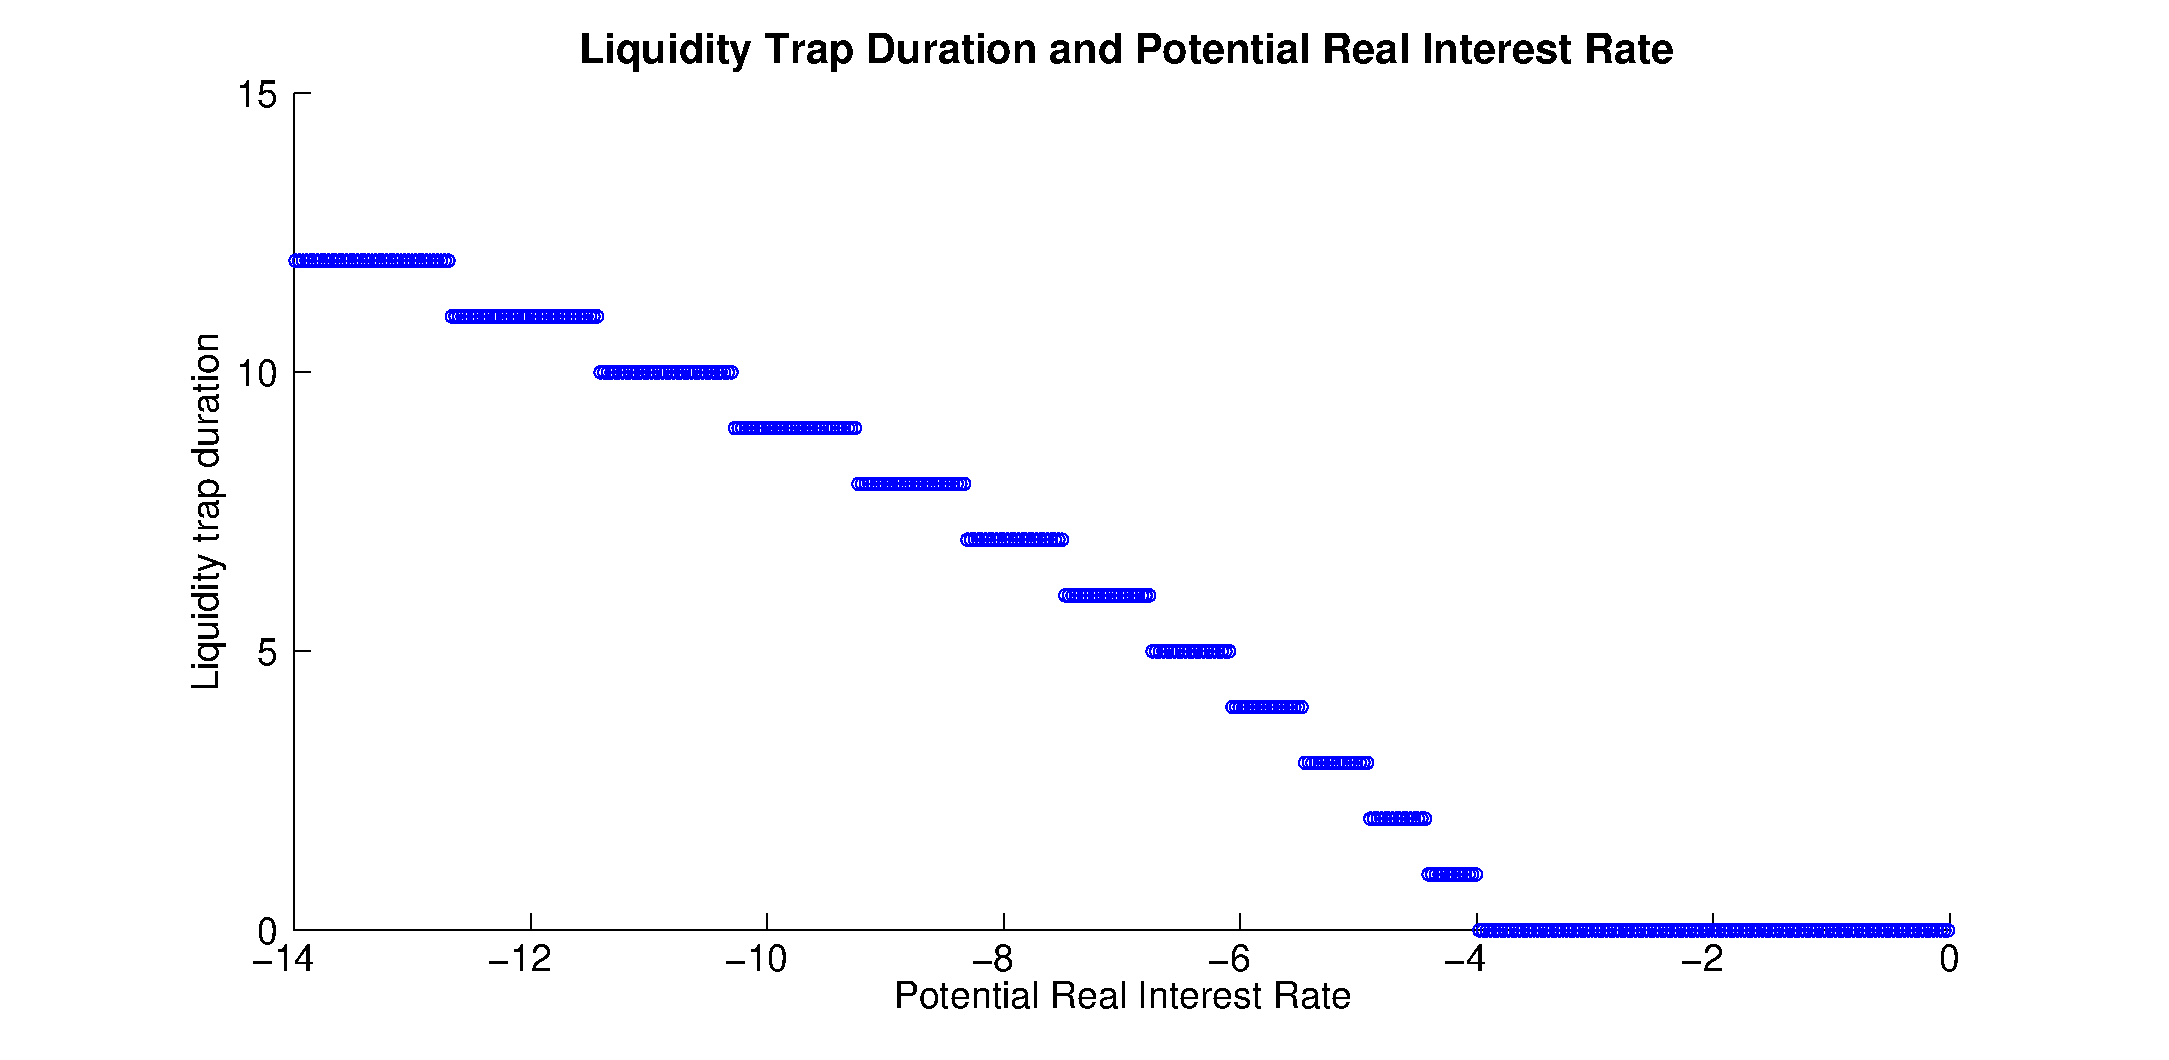
\includegraphics[width=0.8\textwidth]{Paperpics/Figure1bscatter}
\caption{Potential Real Interest Rate and Variation of Taste Shock (Scatter plot)}
\label{Figure1bscatter}
\end{figure}


\subsection*{The Calvo Price Setting}
The slope of the Phillips curve is one important factor in the analysis of the government spending multiplier and the impact of fiscal spending on government debt. In Figure \ref{IRnoinflation}, we begin with an environment of zero inflation.
As the inflation is kept to zero, the annualized real interest rate falls to $-4\%$ and follows the path of the nominal interest rate $\left(r_t = i_t\right)$. We change the Calvo parameter to 0.8 to get a 5 quarter price contract duration in the model and thereby allow inflation to react. When the economy now hits the zero lower bound and inflation is responsive, the fall in output is very large. The exogenous shock leads to a fall in marginal costs and a decline in prices, which changes the inflation expectations of the agents. Real interest rates have then to rise when the nominal interest rate is stuck at the zero lower bound. Consequently, households change their consumption behavior by increasing their savings, which reduces the output even further.
\par
\bigskip
At the zero lower bound monetary policy cannot cut the nominal interest rate far enough. With falling inflation the real interest rate rises, triggering an even stronger fall in output. When the nominal interest rate hits the lower bound, the central bank does not have any further options to react in our simple model. We see therefore that the real interest rate plays the key role at the ZLB in the NK model. In this framework fiscal policy becomes crucial to stabilize the economy and counteract the negative taste shock. Figure \ref{IR5quarter} illustrates these results.

\begin{figure}[!th]
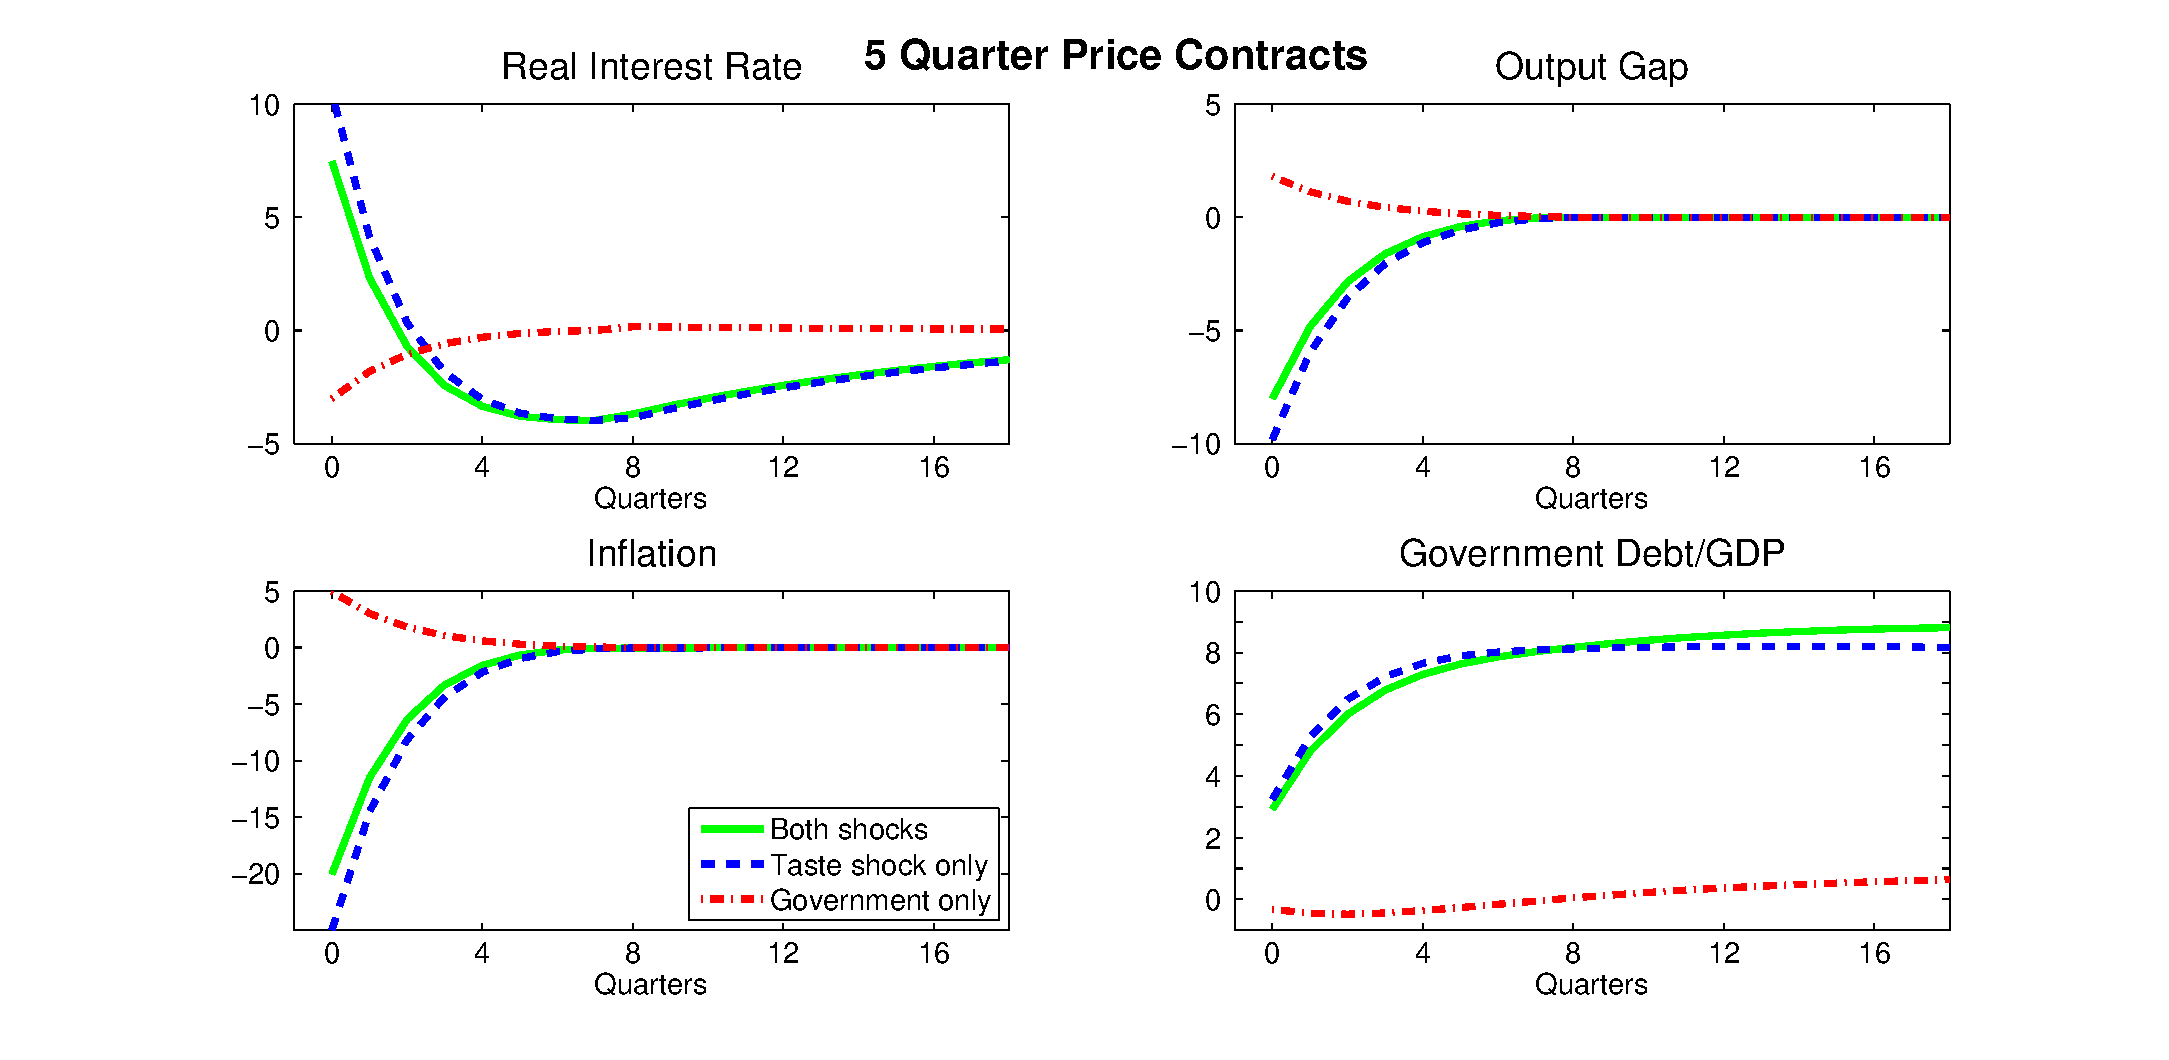
\includegraphics[width=\textwidth]{Paperpics/Figure25quarter}
\caption{Immediate Rise in Government Spending (5 Quarter Price Contracts)}
\label{IR5quarter}
\end{figure}


\subsection*{Policy rules}
In the following, we shift the focus to the monetary and fiscal policy rules. After setting the parameters of the monetary rule in Figure \ref{IR5quarter} arbitrarily large, we change the monetary policy rule to values that are more \textit{usual} in standard New Keynesian models. We set the Taylor rule parameter on output $\gamma_x$ to 0.2 and inflation $\gamma_{\pi}$ to 1.5. As a result the negative taste shock leads to an explosive behavior of the impulse response. The amplitude reaches boundaries that are unrealistic and not useful for further economic analysis. The careful calibration of the Taylor rule parameter must be seen as essential in our model and part of an optimal monetary policy analysis.

\begin{figure}[!th]
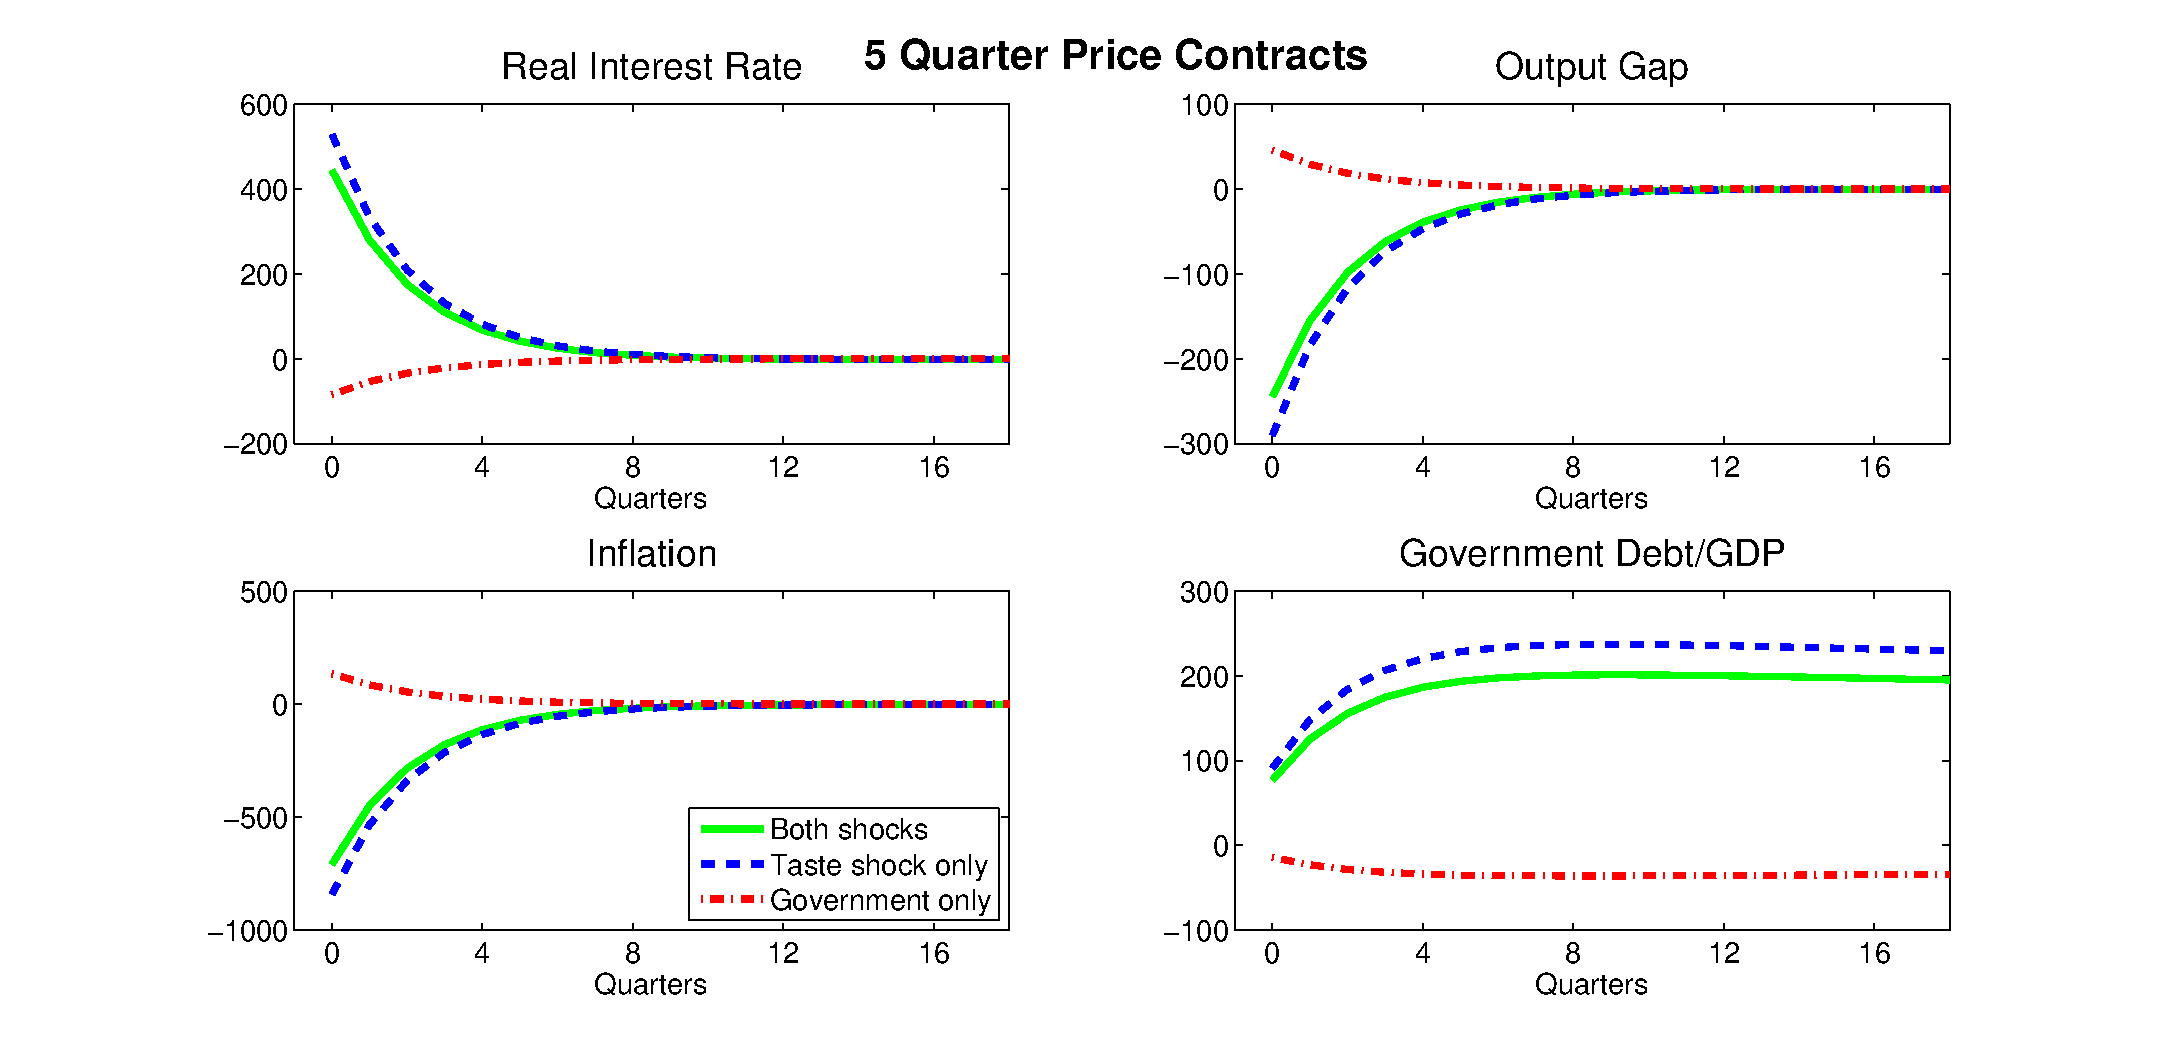
\includegraphics[width=\textwidth]{Paperpics/Figure25quarternewtaylorrule}
\caption{Immediate Rise in Government Spending (Alternative Taylor Rule Values)}
\label{IR5quarternewtr}
\end{figure}

We turn the focus now to the fiscal response. Figure \ref{Figure1a} shows how the rise in government spending helps to shorten the liquidity trap duration. The negative taste shock leads to a fall in the potential real interest rate and keeps $r^{pot}$ below the nominal interest rate for eight quarters. Fiscal policy partly offsets this drop and pushes the potential real interest rate upwards. Nevertheless, the spending increase of $1\%$ of total GDP is still not high enough to shorten the liquidity trap duration. As the fiscal response exceeds a certain threshold, the liquidity trap duration decreases to seven quarters. That is exactly the case with the $2\%$ spending hike. It is big enough to reduce the duration of the liquidity trap by one period, which enables the central bank to raise the nominal interest rate after seven quarters.

\begin{figure}[!th]
\centering
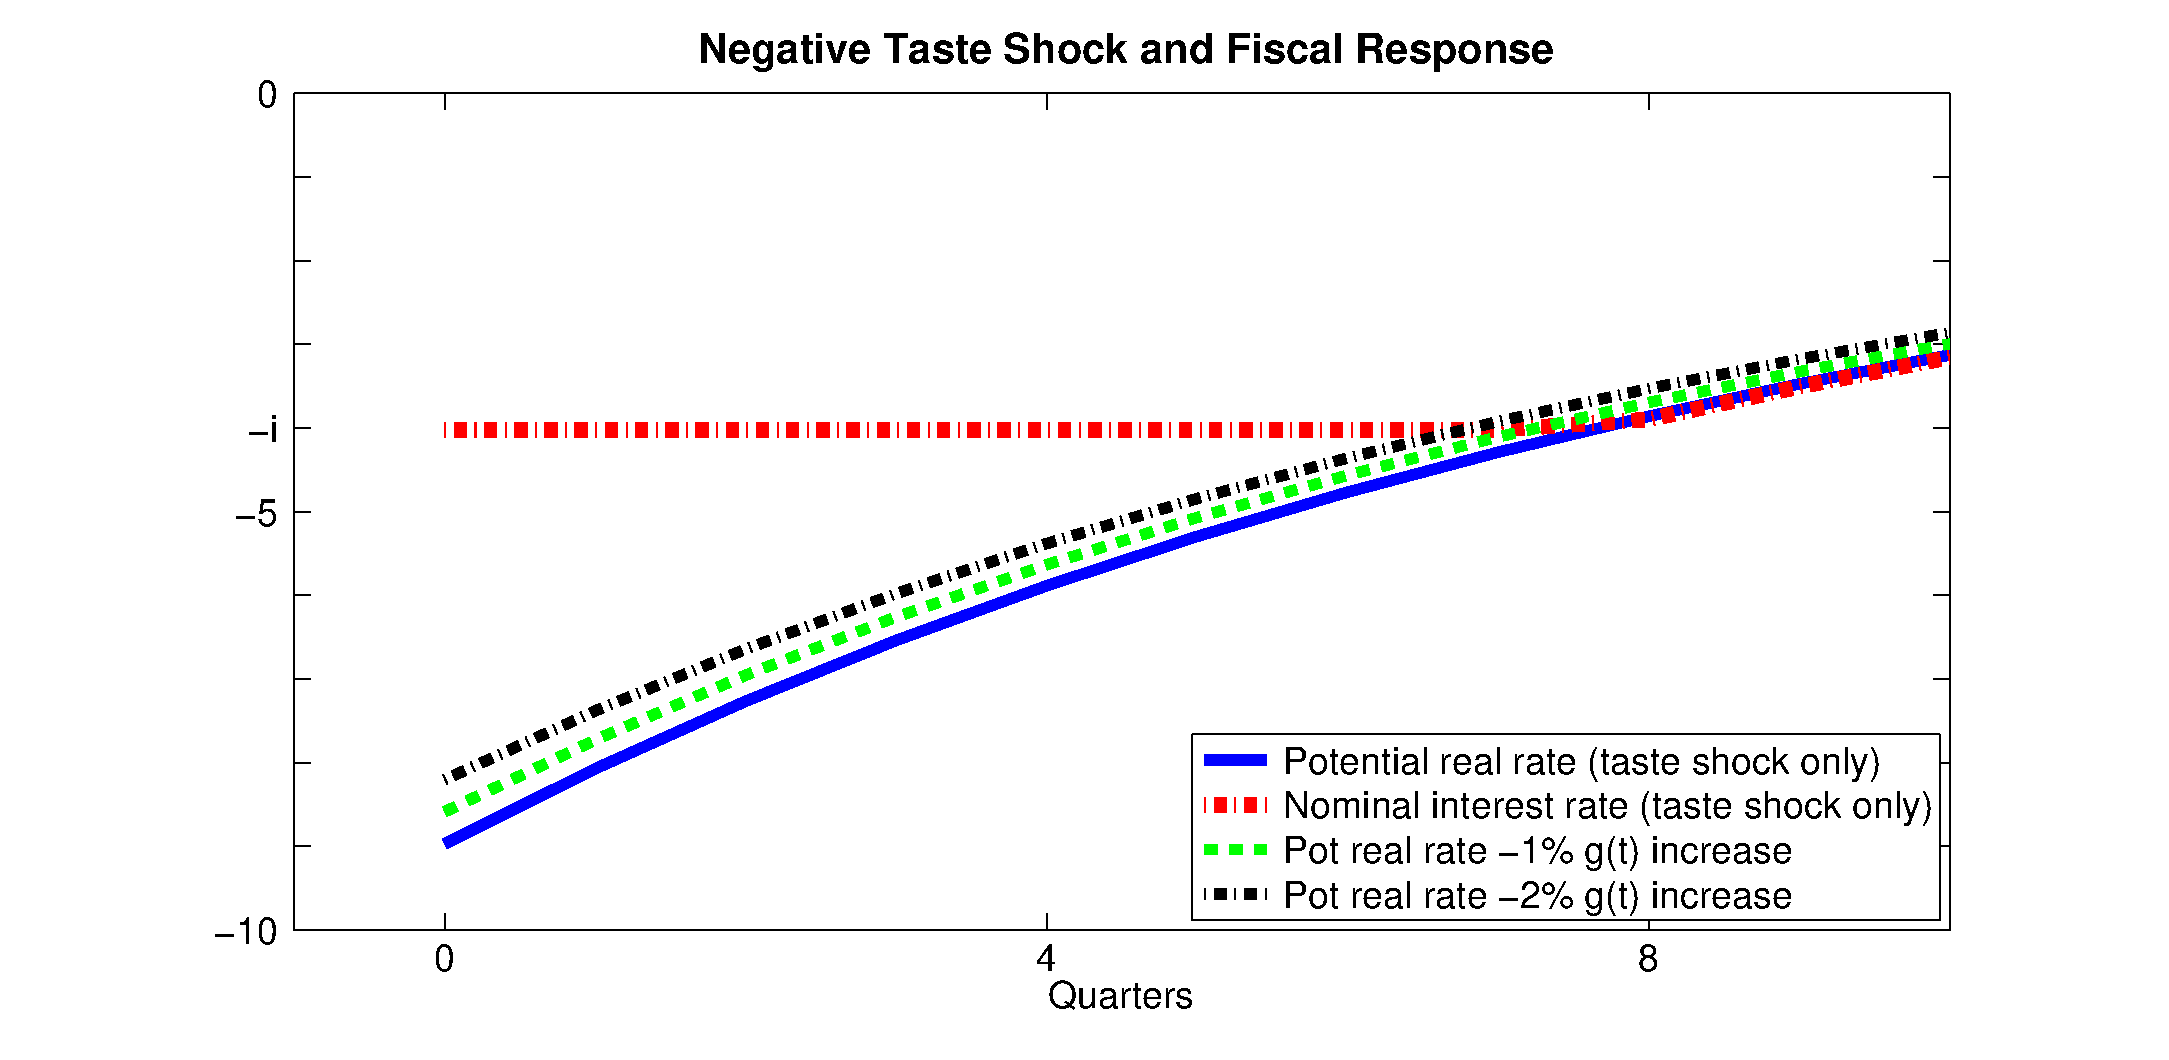
\includegraphics[width=0.8\textwidth]{Paperpics/Figure1a}
\caption{Potential Real Interest Rate and Fiscal Response}
\label{Figure1a}
\end{figure}



\input{Multiplier}
\section{Workflow}

\subsection*{GitHub}
\label{sub:GitHub}

To coordinate and control our coding, we have used GitHub\footnote{https://github.com}. GitHub is version control software based on the git system. It allows its users to keep track of all the changes made to a specific project and provides an overview of the its development. GitHub has a variety of features and it is mostly used by software engineers who work simultaneously with many other people in big projects. GitHub was particularly useful to us because it forced us to document all the changes we made to the project. This way it was much easier for us two to work remotely without losing track of what each other had already done.

Alongside with the documentation function, the git system offers the possibility to reload previous versions of the project and undo changes that turn out to be undesired. GitHub displays a timeline in which the user can follow the development of the project from its beginning until its current state. This allows the user to go back in time and recover old versions of project or only parts of it. This was particularly useful for us too. It happened more than once that one of us two has mistakenly changed the code and Dynare could no longer simulate the model. Instead of spending hours debugging and trying to find the error, we simply opted to go back to a previous version and start again from there.

Although the git system is primarily designed to be used from the command line (Terminal for macOS or Command Line for Windows), GitHub offers a very user-friendly desktop application, which makes possible for not-so-advanced user to profit from its features. GitHub is free as long as you are willing to make your project public. The code for this project, for example, is available online \footnote{https://github.com/denismaciel/fiscalfreelunch}.


\subsection*{Syntax Highlighting}
\label{sub:Syntax Highlighting}

Another tip worth mentioning is to use syntax highlighting while coding. It is not only much more comfortable to read a code whose parts have different colors according to its function, but the task of spotting errors becomes much easier when the code is highlighted. Even though we could not find a specific syntax highlighting package for Dynare, it turns out that Java's highlighting works well with Dynare. For example, \% is used to comment the code and that single feature makes worth trying it.




\section{Conclusion}
The paper makes a strong case for the effectiveness of government spending in a liquidity trap, even if it warns against the fact that this effectiveness, measured by the marginal multiplier, may decline at a fast rate. It is important, however, not to forget the assumptions the model rests on. The taste shock that pushes the economy down to the zero lower bound, for example, implies a decrease of $23\%$ of GDP. Such a decline in output does not occur very often in real economies. For that reason, a very thorough assessment of the real economy should done to check if the model can adequately inform policy-making for it. 
\par
\bigskip
In general lines, we have been able to replicate the most important results of \citet{Erceg.2014}. Even when we could not get the exact values, our simulations behaved qualitatively in the same way as in the original paper. The results from the paper and from our replication are most different in the scenario with no inflation. For example, we got a multiplier that is roughly 0.1 smaller. In scenarios with Calvo parameter different than one, it seems we managed to get the exact same results of the paper (judging from the plots). 
\par
\bigskip
The results of the model are very interesting and point to new research questions that could well be answered by refining the baseline model. Due to the importance of the Calvo parameter and the price setting framework in the model, alternative analysis with prices adjustments according to sticky information, rational inattention or state-dependent price settings are interesting for further research. Moreover, the simple New Keynesian model can be expanded to include a negative debt position in the steady-state, an open economy framework, the distinction between tax and debt financed government spending and an empirical comparison between the US and the euro area.    



\pagebreak[4]
\addcontentsline{toc}{section}{References}
\bibliographystyle{plainnat}  %Zitationsstil
\bibliography{References}



%Tabellen
\newpage

\begin{table}[th]
\centering
\caption{Parameter Values Benchmark Calibration}
\bigskip
\bgroup
\def\arraystretch{1.5}
\begin{tabular}{p{1.2cm} l c}
\toprule\toprule \noalign{\smallskip}
 & \multicolumn{1}{c}{\textit{Description}} & \textit{Value} \\
\hline\noalign{\smallskip}

$\alpha$ & Capital Share   & 0.3 \\
$\beta$  & Discount Factor & 0.995 \\
$\sigma$ & Intertemporal Substitution Elasticity & 1 \\
$\chi$ & Inverse of Frisch-Elasticity & 2.5 \\
$g_y$ & Government Share on Output & 0.2 \\
$\varphi_b$ & Tax Rule Parameter & 0.01 \\
$\nu_c$ & Scale Parameter on the Taste Shock & 0.01 \\
$\rho$ & AR(1) Natural Rate for both Shocks & 0.1 \\
$\xi_p$ & Calvo Parameter (No Inflation) & 1 \\
 & Calvo Parameter (10 quarter price contracts) & 0.9 \\
 & Calvo Parameter (5  quarter price contracts) & 0.8 \\
 & Calvo Parameter (4  quarter price contracts) & 0.75 \\
 & Calvo Parameter (3  quarter price contracts) & 0.667 \\
$\gamma_{\pi}$ & Taylor Rule Coefficient on Inflation & 66.15 \\
$\gamma_x$ & Taylor Rule Coefficient on Output Gap & 66.15 \\
 & Taylor Rule Coefficient on Output Gap (Figure \ref{IRnoinflation}) & 15 \\
\bottomrule
\end{tabular}
\egroup
\label{tab:Tabel1}
\end{table}


\end{document}
